\documentclass[varwidth]{standalone}

\usepackage[]{graphicx}
\usepackage{subfigure}

\begin{document}
\begin{figure}
  \centering
  \hspace*{\fill}
  \subfigure[]{\label{subfig:1a}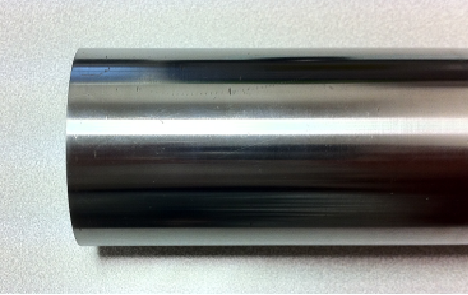
\includegraphics[width=0.15\linewidth]{A1.png}} \hfill
  \subfigure[]{\label{subfig:1b}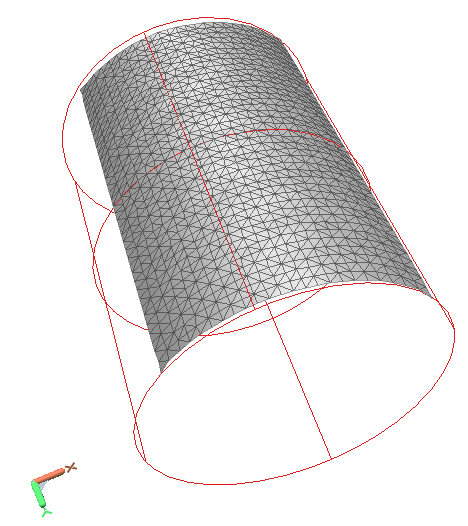
\includegraphics[width=0.15\linewidth]{A2.png}} \hfill
  \subfigure[]{\label{subfig:1c}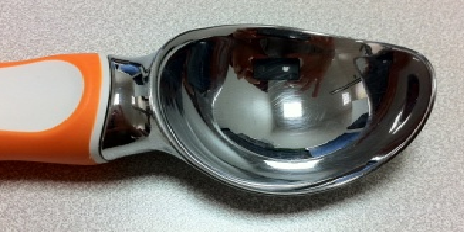
\includegraphics[width=0.15\linewidth]{B1.png}} \hfill
  \subfigure[]{\label{subfig:1d}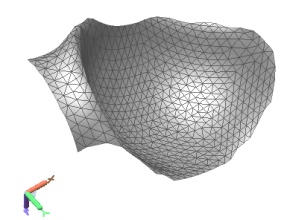
\includegraphics[width=0.15\linewidth]{B2.png}}
  \hspace*{\fill} \\ \hspace*{\fill}
  \subfigure[]{\label{subfig:1e}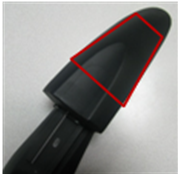
\includegraphics[width=0.15\linewidth]{C1.png}} \hfill
  \subfigure[]{\label{subfig:1f}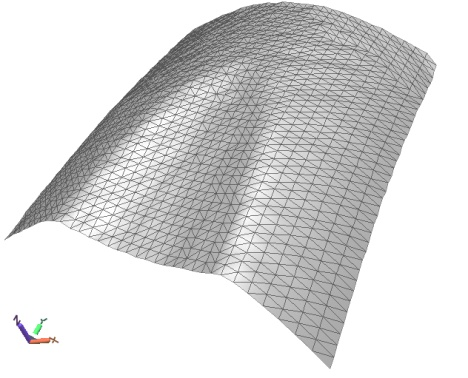
\includegraphics[width=0.15\linewidth]{C2.png}} \hfill
  \subfigure[]{\label{subfig:1g}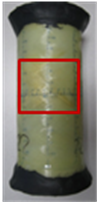
\includegraphics[width=0.1\linewidth]{D1.png}} \hfill
  \subfigure[]{\label{subfig:1h}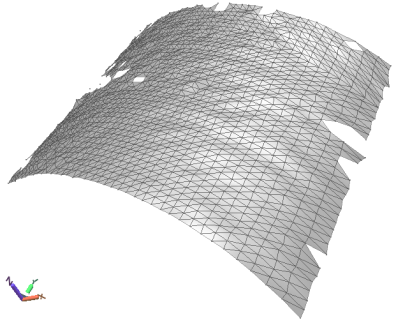
\includegraphics[width=0.15\linewidth]{D2.png}}
  \hspace*{\fill} \\ \hspace*{\fill}
  \subfigure[]{\label{subfig:1i}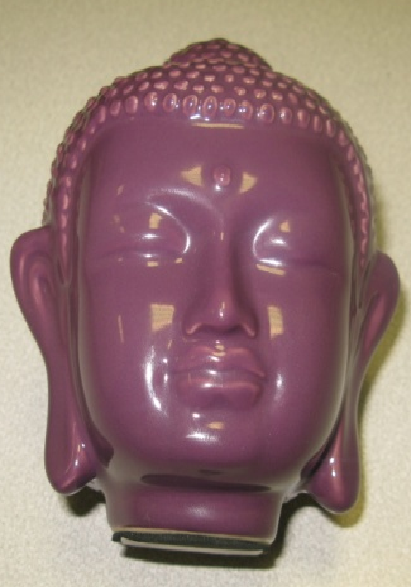
\includegraphics[width=0.15\linewidth]{E1.png}} \hfill
  \subfigure[]{\label{subfig:1j}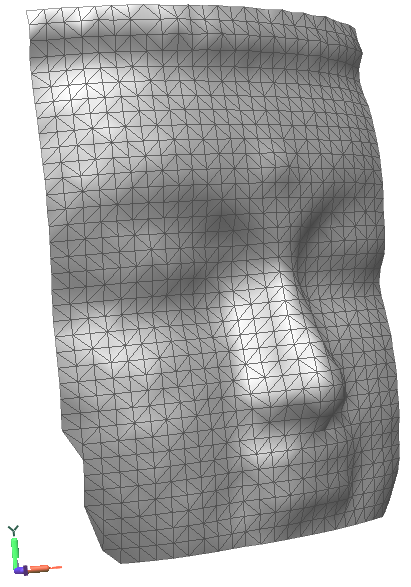
\includegraphics[width=0.15\linewidth]{E2.png}} \hfill
  \subfigure[]{\label{subfig:1k}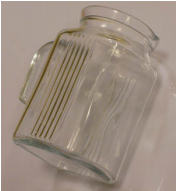
\includegraphics[width=0.15\linewidth]{F1.png}} \hfill
  \subfigure[]{\label{subfig:1l}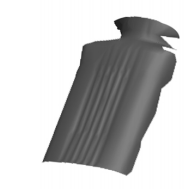
\includegraphics[width=0.15\linewidth]{F2.png}}
  \hspace*{\fill}
	  % \caption{Examples of 3D digitization obtained by \acs*{sfh} approach: (a), (b), (c) and (d) metallic specular surfaces \cite{bajard2013numerisation} - (e) and (f) black plastic - (g) and (h) composite material - (i) and (j) ceramic - (k) and (l) glass transparent object \cite{meriaudeau20113d}.}
  % \label{fig:1}
\end{figure}
\end{document}
